\section{Graph-based Problem Formulation Syntax}
We begin by discussing the general syntax of graph theory and then expand upon this syntax to represent the data flow of an MDAO problem.
A graph is a pair $G = (V,E)$ of sets such that $E \subseteq V \times V$, which means that the elements of $E$ are 2--element subsets of $V$ \cite{Diestel2010}. 
For a directed graph we construct $E$ as a set of ordered pairs instead of a set of sets. Each ordered pair represents an edge starting at the node indicated by the first entry and directed to the node indicated by the second entry. While $E$ is effectively a mapping from $V$ to $V$, we reference this mapping as $e$.
\begin{figure}[htb!]
	\begin{center}
	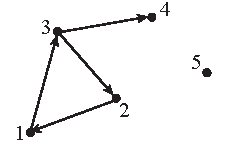
\includegraphics[width=1.5in]{images/example_directed_graph}
	\end{center}
	\vspace{-20pt}
\caption{Example directed graph.}
\label{f:example directed graph}
\end{figure}
As an example, for the directed graph shown in Fig.~\ref{f:example directed graph} we have
\begin{IEEEeqnarray*}{rCl}
V & = & \{1,2,3,4,5\}, \\
E & = & \big\{(1,2),(3,2),(1,3),(3,4)\big\}.
\end{IEEEeqnarray*}

We now assign additional properties to the nodes and edges so that they may represent the data flow of an MDAO problem. 
The first property assigned to nodes and edges is the \emph{type}. The possible node types are:
\begin{description}
\item[input] The `input' node has specific rules for the number of edges that may be directed into it.
\item[simple] The `simple' node has no additional properties and is used as a building block.
\end{description}

The possible edge types are:
\begin{description}
\item[connection] The `connection' edge represents the passing of data between analysis blocks.
\item[data] The `data' edge represents the passing of data within an analysis block.
\item[analysis] The `analysis' edge contains additional properties to represent the execution of an analysis block.
\end{description}
Then, considering sets $T_\txt{node}$ and $T_\txt{edge}$ to be sets containing the possible node types and edge types, respectively, we use mappings $t_\txt{node}:V \to T_\txt{node}$ and $t_\txt{edge}:E \to T_\txt{edge}$ to assign a type to each node and edge. Nodes and edges are herein referred to by their type (e.g. `connection' edge). Additional properties will be discussed in subsequent sections.

Next, we introduce the graph $A$ which represents a single analysis block broken down into its individual inputs and outputs. An example graph is shown in Fig.~\ref{f:analysis block} to demonstrate the basic structure. This structure is derived from the need to represent each input and output individually while representing the actual analysis with a single node or edge. The `input' nodes each represent a single input of the analysis block. Each of these nodes is connected to a single `simple' node via a `data' edge, which represents the gathering of the inputs to begin the analysis. Next the `simple' node is directed to another `simple' node via the `analysis edge', which represents the actual analysis. Finally, this `simple' node is directed to several `simple' nodes via individual `data' edges, and this represents individual local outputs which may then be connected to other analysis blocks.
\begin{figure}[htb!]
	\begin{center}
	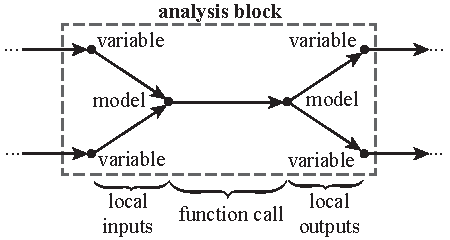
\includegraphics[width=4in]{images/analysis_block}
	\end{center}
	\vspace{-20pt}
\caption{Example directed graph. The each node type and edge type is labeled, with nodes being label in italics.}
\label{f:analysis block}
\end{figure}
`Connection' edges connect the local outputs from one analysis block to input nodes. In this way, the analysis block graph is the fundamental building block of the MDAO problem data flow.

\subsection{Maximal Connectivity Graph}
Next, Consider an MDAO problem defined by a set of codes, global inputs, global outputs. The codes are represented by analysis blocks $A_i=(V_{A_i},E_{A_i}), \ i=1,\ldots,m$, the global inputs are represented a set of `simple' nodes $I$, and the global outputs are represented by a set of `input' nodes $O$. We assume that $O$, $I$, and $A_i$ are given, and that any potential connection edge is given in the form of the set $C_M$. 
Then we may construct the \emph{maximal connectivity graph} $M=(V_M,E_M)$ as
\begin{IEEEeqnarray*}{rCl}
V_M & = & I \cup O \cup \left( \bigcup_{i = 1}^m V_{A_i} \right), \\
E_M & = & C_M \cup \left( \bigcup_{i=1}^m E_{A_i} \right).
\end{IEEEeqnarray*}
The maximal connectivity graph contains all possible connections that may exist between the given analysis blocks.

\subsection{Fundamental Problem Formulation Graph}
Before defining the the fundamental problem formulation graph, let us first define $\txt{deg}^-(v)$ as the \emph{indegree} $\txt{deg}^+(v)$ as the \emph{outdegree} of vertex $v$, where indegree and outdegree refer to the number of edges directed into vertex $v$ and the number of edges directed out of vertex $v$, respectively. Then, define a mapping $d:V \to \mathbb{N}$ to specifiy the maximum number of connections that are allowed into an input node.
If $d(v)>1$ for an input node, this means that multiple inputs are accepted, such as the case for a multifidelity formulation.

% Next, let $H$ be the set of all nodes which are \emph{holes} in $M$ and define $H$ as
% \begin{equation}
% H=\big\{v \in M \big| t_\txt{node}(v) = \txt{`local input' or `global output'} \txt{ and } \txt{deg}^-(v) = 0\big\}.
% \end{equation}
% Also, let $L$ be the set of all nodes which are \emph{collisions} in $M$ and define $L$ as
% \begin{equation}
% L = \big\{v \in M \big| t_\txt{node}(v) = \txt{`local input' or `global output'} \txt{ and } \txt{deg}^-(v) > d(v) \big\}.
% \end{equation}
We may now define the \emph{fundamental problem formulation graph}, $F=(V_F,E_F)$, as a directed graph meeting the following conditions
\begin{enumerate}
\item[(1)] $\displaystyle{V_F = I_F \cup O \cup \left( \bigcup_{i \in \mathcal A} V_{A_i} \right),\ I_F \subset I}$
\item[(2)] $\displaystyle{E_F = C_F \cup \left( \bigcup_{i \in \mathcal A} E_{A_i} \right)}$
\item[(3)] $\displaystyle{\forall v \in V_F \txt{ with } t_\txt{node}(v) = \txt{`input,'}\quad 0 < \txt{deg}^-(v) \leq d(v)}$
\end{enumerate}
The set $\mathcal A$ is an index set containing the indices of the analysis blocks in $F$. The first requirement for $F$ is that $V_F$ be composed of all of the global outputs (which are given as required), the nodes from each analysis block in $F$, and any global input nodes that are needed, $I_F$. The second requirement suggests that the edges in $F$ comprise the edges for each analysis block and the connections between them, the global inputs, and the global outputs. The final requirement is specific to the number of connection edges directed into a local input node or a global outputs node. If there are no connections directed inward, the node is called a \emph{hole}, and if more connections are directed in than are allowed, the node is called a \emph{collision}. The final requirement is therefore a requirement on $C_F$.

\subsection{Obtaining the Fundamental Problem Formulation Graph}
In general, there may be multiple different graphs that satisfy the FPF conditions, though there may be none at all. Here, we describe a process for obtaining an FPF by starting with the MCG and removing nodes and edges until the FPF conditions are met. Then the problem is reduced to deciding which nodes and edges to remove, and this is centered on the input nodes, which are treated as decision switches.

Then, mathematically, the FPF starts with $\mathcal A_1 = \{1,\ldots,m\}$, $I_{F,1} = I$, and $C_{F,1} = C_M$.



\begin{enumerate}
\item The first step is to detect holes and remove the corresponding analysis blocks, which could not be used because the required inputs are not supplied. Any analysis blocks with holes may be stored in an index set $\mathcal H$ as
\begin{equation}
\forall i \in \mathcal A_1,\txt{ and }\forall v \in V_{A_i},\txt{ if deg}^-(v)=0 \txt{ then } i \in \mathcal H.
\end{equation}
Then an updated index set $\mathcal A_2$ is created using set difference notation as
\begin{equation}
\mathcal A_2 = \mathcal A_1 \setminus \mathcal H
\end{equation}The connection edges directed from the removed analysis blocks are removed as
\begin{equation}
H = \{c \in C_{F,1} |c = (e^{-1}(v),v), \txt{ where } v \in V_{A_i} \txt{ for some } i \in \mathcal H\},
\end{equation}
\begin{equation}
C_{F,2} = C_{F,1} \setminus H
\end{equation}
Finally, the FPF is updated as
\begin{equation}
V_{F,2} = I_{F,2} \cup O \cup \left( \bigcup_{i \in \mathcal A_2} V_{A_i} \right),
\end{equation}
\begin{equation}
E_{F,2} = C_{F,2} \cup \left( \bigcup_{i \in \mathcal A_2} E_{A_i} \right)
\end{equation}
This process may require multiple iterations because removing an analysis block may create holes upstream. It is assumed that the process as been repeated sufficiently such that $\mathcal A_2$ does not have any holes.

\item The next step is to resolve conflicts. The set $C$ of input nodes containing conflicts is
\begin{equation}
C = \{v \in V_{F,2} | t_\txt{node}(v) = \txt{`input'} \txt{ and } \txt{deg}^-(v) > d(v)\}
\end{equation}
%\begin{equation}
%for v \in c let 
%\end{equation}
\end{enumerate}

\subsection{Classification of the FPF}

%A collision represents a choice.
%Delete edges and analysis blocks so that there are no nodes or collisions.





% \begin{figure}[htb!]
	% \begin{center}
	% 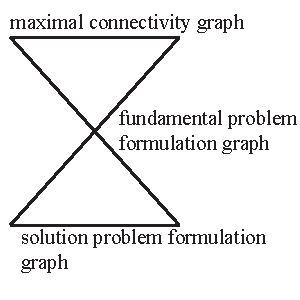
\includegraphics[width=2in]{images/hour_glass}
	% \end{center}
	% \vspace{-20pt}
% \caption{(()).}
% \label{f:our glass}
% \end{figure}
% \subsection{old}
	% For a large scale problem with many analyses, obtaining the FPF is likely to be a challenge. In general, a set of analysis codes will be given and the desired outputs will be specified as
	    % \begin{align}
            % given & \ \ A: \lbrace x_i \lvert i \in A_\textrm{input} \rbrace \rightarrow \lbrace x_i \lvert i \in A_\textrm{output} \rbrace \notag
            % \\    & \ \ B: \lbrace x_i \lvert i \in B_\textrm{input} \rbrace \rightarrow \lbrace x_i \lvert i \in B_\textrm{output} \rbrace \notag
			% \\    & \ \ \quad \quad \quad \quad \quad \quad  \quad \quad \vdots
            % \\min. &\ \ f(x_i), i \in \mathcal{O} \notag
            % \\w.r.t. & \ \ x_i, i \in \mathcal{I}, \notag
            % \label{eqn:preFPF}
        % \end{align}
	% where $\mathcal{O}$ is the index set of the global outputs and $\mathcal{I}$ is the index set of the global inputs. For this to be an FPF, there must be no \emph{conflicts} or \emph{holes}. A conflict arises when different analyses produce the same output; two analysis codes $A$ and $B$ are in conflict if
		% \begin{equation}
			% A_\textrm{output} \cap B_\textrm{output} \neq \emptyset.
		% \end{equation}
	% A hole arises when a local input to an analysis block is neither a global input nor a local output of any analysis block. If we let $\mathcal{H}$ denote the index set of local inputs which are holes
		% \begin{equation}
			% i \in \bigcup \{A_\textrm{input},B_\textrm{input},\ldots\} \textrm{ and } i \notin \bigcup \{\mathcal{I},A_\textrm{output},B_\textrm{output},\ldots\}  \implies  i \in \mathcal{H}.
		% \end{equation}
	% If the given set of analyses contains any holes, an FPF cannot be obtained. On the contrary, if there are conflicts multiple FPFs may be obtained. This is because every conflict represents a choice of which analysis to use and each choice could (potentially) yeild a different but valid FPF. The following section develops an application of graphy theory to obtain multiple FPFs from a set of analyses and desired outputs.
		
    % \subsection{Formulation Graph Syntax}
    % Rather than start with an adjacency, we chose to work directly with a directed cyclic graph to develop a syntax for the FPF. 
    % The following information must be provided to start:
    % \begin{itemize}
        % \item Analysis blocks: an analysis block represents any calculation, and each comes with
            % \begin{itemize}
                % \item local inputs
                % \item local outputs 
                % \item execution properties: these are the properties associated with running the code, such as run time
            % \end{itemize}
        % \item Global parameters: these may serve as fixed inputs to the local inputs of analysis blocks
        % \item Global outputs: these may represent
            % \begin{itemize}
                % \item objectives
                % \item constraints
                % \item residuals: (not sure)
            % \end{itemize}
    % \end{itemize}

    % The graph representation of a data flow is cast to utilize the extensive library of algorithms in graph theory to analyze a directed weighted graph. 
    % Edge weights are used to represent the metrics associated with a data flow:
    % \begin{itemize}
        % \item Run time: this metric is a property of an analysis block
        % \item Fidelity: this metric is a property of an individual local output
        % \item Expected Convergence
    % \end{itemize}

    % The key assumption is that identical variables are recognized as such. This serves as the basis for creating a data flow by connecting compatible input and output nodes with a directed edge. 
    % To represent the fact that execution of an analysis code does not depend on the number of outputs being used, we have created the following figure (not made yet).
    
    % This information immediately leads to the maximal connectivity graph, which is formed by placing a directed edge from each local output or global parameter to each matching local input or global output. 
    % Whenever multiple edges are connected to a single input, a conflict occurs because only one may be used. Resolving these conflicts is one key challenge in creating a data flow.
%    \begin{itemize}
%        \item Specify analyses
%        \item Connections between analyses 
%            \begin{itemize}
%                \item local variables
%                \item global variables? Use "fake" node that broadcasts out to the rest of the graph? 
%            \end{itemize}
%        \item Cycles indicate coupling
%        \item Cycles for design variables->objectives/constraints
%        \item Objectives/constraints are just outputs? Special nodes? 
%        \item Residuals are just outputs? Special nodes? 
%        \item Parameters are just input nodes that are not design variables (use identifies these)
%        \item FPF no solvers/optimizers anywhere in it
%    \end{itemize}

    \subsection{Solution Graph Syntax}
    What is the difference between a problem formulation and a problem solution method? Convert from a cyclic graph, to an acyclic graph
    \begin{itemize}
        \item Cycles indicate convergence loops or design variable loops
        \item Problem can't be solved until all loops are *removed* by adding solvers/optimizers
        \item *Special* nodes for solvers and optimizers that *break* loops (from an algorithmic point of view)
        \item FPF represents the minimal amount of information necessary to define a problem
        \item Any solution path grows the graph complexity by adding edges and nodes (or possibly have an empty solution graph, which you build up
        as you remove edges from problem formulation graph?)
    \end{itemize}
